\documentclass[a4paper]{article}
\usepackage {changepage}
\usepackage{fancyhdr}
\usepackage {fontspec}
\usepackage {paralist}
\usepackage {multicap}
\pagestyle{fancy}
\setromanfont{Lantinghei SC Extralight}
\setmonofont{Courier New}
\XeTeXlinebreaklocale ``zh''
\XeTeXlinebreakskip = 0pt plus 1pt
\textheight = 650pt
\begin{document}
\title{实验报告 Lab 5}
\author{姓名:王钦\quad 学号:13349112}
\date{}
\maketitle

\section*{ A look at the captured trace}
\hangindent=4em \hangafter=-200{
	\begin{center} 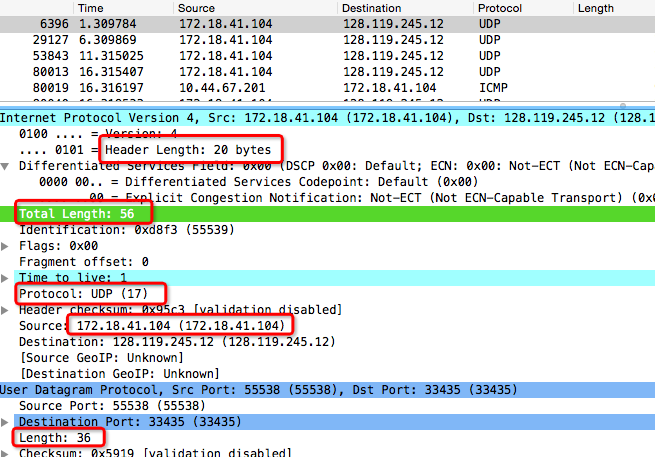
\includegraphics[scale=0.5]{Illustrations/1.png} \mfcaption{UDP segment}\end{center}
	\begin{enumerate}
	\item the IP address of my computer:\verb| 172.18.41.104|,see figure 1.(Note: use tracerout on mac os)
	\item upper layer protocol field:\verb| UDP (17)|,see figure 1
	\item bytes are in the IP header:20 bytes,bytes are in the payload of the IP datagram:36 bytes.Total length:56 bytes.See figure 1
	\item The more fragments bit = 0, so the data is not fragmented.
	\begin{center} 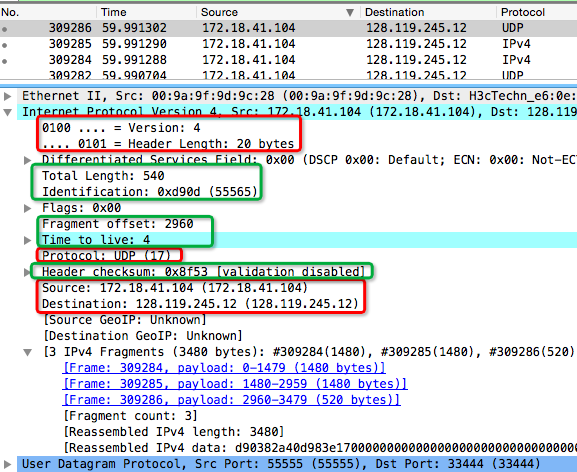
\includegraphics[scale=0.5]{Illustrations/2.png} \mfcaption{Internet Protocol portion}\end{center}
	\item always change:Identification, Header checksum ,fragment offset.some point green rect in figure 2.
	\item Stay constant
		\begin{itemize}
			\item Version (since we are using IPv4 for all packets)
			\item header length (since these are 20 bytes)
			\item source IP (since we are sending from the same source)
			\item destination IP (since we are sending to the same dest)
			\item Differentiated Services (since all packets are UDP they use the same Type of Service class)
			\item Upper Layer Protocol (since these are UDP packets).some point red rect in figure 2.
		\end{itemize}
	   Must constant
		\begin{itemize}
			\item Version (since we are using IPv4 for all packets)
			 \item header length (since these are 20 bytes)
			 \item source IP (since we are sending from the same source)
			 \item destination IP (since we are sending to the same dest)
			 \item Differentiated Services (since all packets are UDP they use the same Type of Service class)
			 \item Upper Layer Protocol (since these are UDP packets),some point red rect in figure 2.
		   \end{itemize}
	 Must change
		\begin{itemize}
			\item Identification(IP packets must have different id)
			\item Time to live (traceroute increments each subsequent packet)
			\item Header checksum (since header changes, so must checksum)
		\end{itemize}
	\item Identification field.The IP header Identification increment with each UDP segment.
	\begin{center} 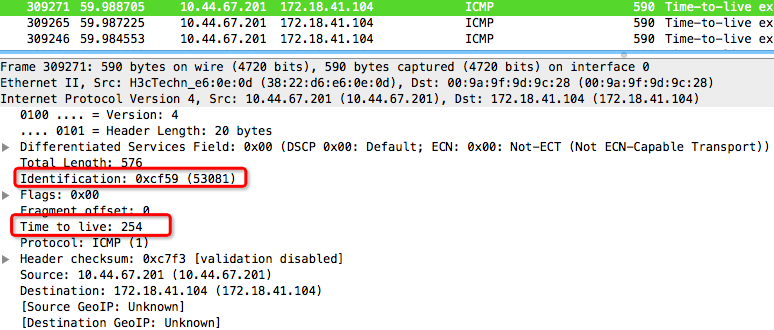
\includegraphics[scale=0.5]{Illustrations/3.png} \mfcaption{ICMP TTL- exceeded replies}\end{center}
	\item Identification :\verb|53081|,TTL:\verb|254|.
	\item Identification always change.But TTL always constant.\\Because the identification field is a unique value for each packets except a case that when two or more IP datagrams have the same identification value, then it means that these IP datagrams are fragments of a single large IP datagram,
	  and the TTL of first hop router is always the same,the distance between my computer and router is constant.
	\item Packet size of 2000 cause fragmentation,see figure 4. 
	\begin{center} 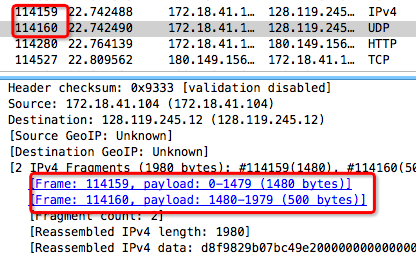
\includegraphics[scale=0.5]{Illustrations/4.png} \mfcaption{2000 bytes fragmentation}\end{center}
	\item From flags field for more fragments is set, indicating the datagram has been fragmented. From fragment offset is 0, incicating this is the first fragment.
	  And total length is 1500.
	\begin{center} 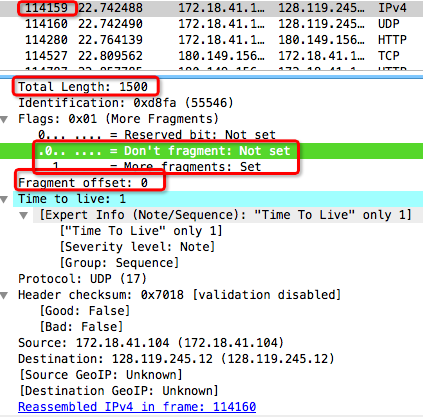
\includegraphics[scale=0.5]{Illustrations/5.png} \mfcaption{first fragment}\end{center}
	\item From fragment offset is 1480 not 0,so isn't first fragment.
	      From flags field for more fragments is not set, indicating the datagram has no more fragments.
	\begin{center} 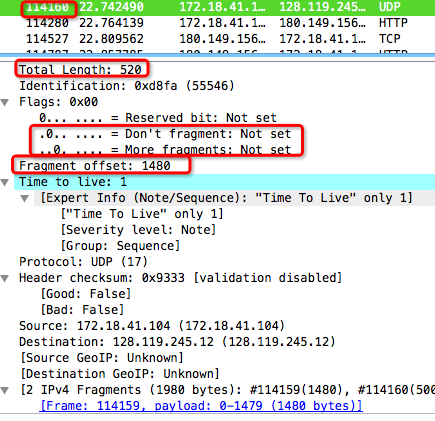
\includegraphics[scale=0.5]{Illustrations/6.png} \mfcaption{second fragment}\end{center}
	\item changed:total length, flags, fragment offset, checksum.some point in green rect see figure 7. 
	\begin{center} 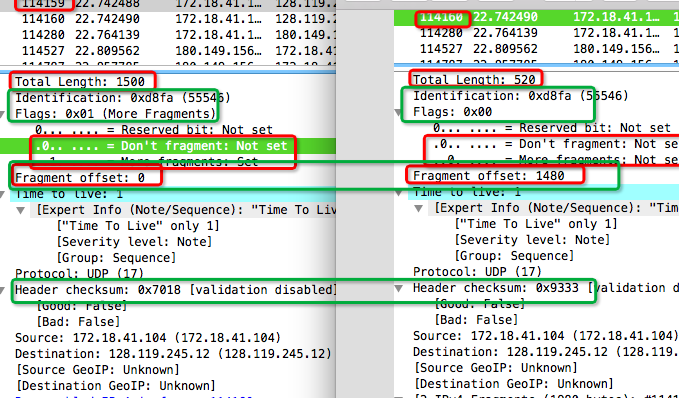
\includegraphics[scale=0.5]{Illustrations/7.png} \mfcaption{changed fields}\end{center}
	\item Packet size of 3500 has 3 fragments see figure 8. 
	\begin{center} 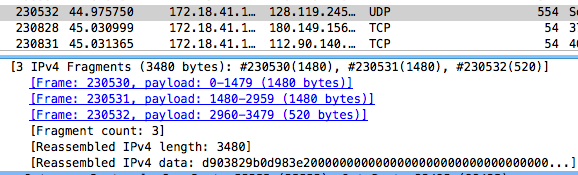
\includegraphics[scale=0.5]{Illustrations/8.png} \mfcaption{changed fields}\end{center}
	\item Fields have changed among the fragments are \verb| Total length, Fragment offset, Header checksum|.\\
	  Detail:
	  \begin{itemize}
		  \item Total length of first fragment and second fragment was the same value 1500,the last is 540.
		  \item Fragment offset of three fragments are\verb| 0, 1480, 2960|.
		  \item Header checksum are unique in each fragment.
	 \end{itemize}
	\begin{center} 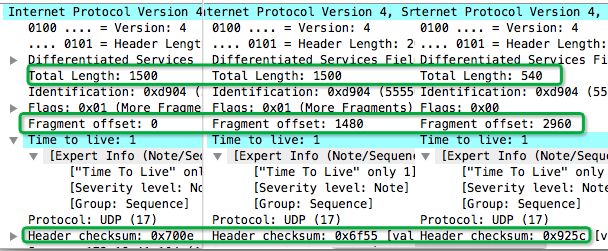
\includegraphics[scale=0.5]{Illustrations/9.png} \mfcaption{changed fields}\end{center}
	\end{enumerate}
}
\end{document}




